\section{Distilling the Knowledge in a Neural Network}

An ensemble of models is a simple method of improving the performance of a machine learning algorithm.
It works by training many different models on the same data and then considering the average of their predictions.
However, an ensemble of models is difficult to incorporate into most end-user devices, because all models 
belonging to the ensemble need to operate to arrive at a useful prediction.

Rich Caruana et al.~\cite{caruana2015compression} have shown it is possible to compress the knowledge
represented by an ensemble of models into a single model with much fewer parameters. This process, called
Knowledge Distillation, allows creating 'specialist' models which are much easier to deploy widely.

The reason an ensemble of models generalizes so well on large datasets is because the average results of the entire 
ensemble is considered. The dataset could possibly contain noise and outliers, but an ensemble manages to avoid overfitting 
because of taking the average of all the model outputs. We cannot expect a smaller model to generalize to large 
datasets without heavy feature engineering, removing many features from the dataset to help the smaller model cope.

The process of knowledge distillation requires us to find 'soft targets'. A soft target is a prediction made by the 
ensemble of models for an input. Unlike hard targets (i.e. targets that are difficult to make sense of), 
soft targets need to have high entropy and low variance in order to provide much more information per training case.

\begin{figure}[h]
    \begin{center}
        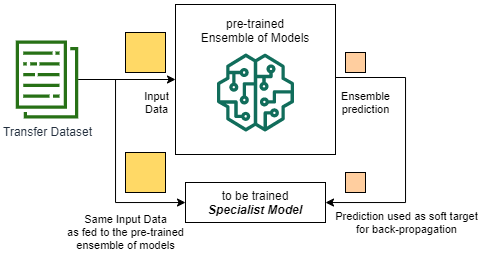
\includegraphics[width=10cm]{KnowledgeDistillation.png}
    \end{center}
    \caption{An illustration of the process of training a specialist model using Knowledge Distillation.
    The specialist models can thus be trained fast, and in parallel.}
    \label{fig:distillation}
\end{figure}

As can be seen in figure~\ref{fig:distillation}, we feed the same training/transfer input 
from the transfer dataset into both the specialist model and the ensemble of models. 
The output of the ensemble of models is then used as a soft target to the specialist model.
The specialist model can thus be trained rapidly, and multiple specialist models can also 
be trained and tested in parallel, and on much higher learning rates, unlike Mixture of Experts, 
where multiple models are learning only a specific part of the dataset, assigned to the models 
based on a gating network mechanism.

\subsection{Discussion}

Geoffrey Hinton et al.~\cite{hinton2015distilling} were able to train large, highly regularized
ensemble of models on various tasks, including the MNIST handwritten digit dataset and Speech 
Recognition deep acoustic models similar to the one used by Android voice search. Nearly all of the 
improvement achieved by training an ensemble of deep neural nets could be trained into a single specialist
model of the same size, achieving similar results, and being easier to deploy to end-user devices.

From these findings, we can thus attempt training smaller specialist models using existing pre-trained models.
These smaller models can thus be deployed widely.